\documentclass{article}

\usepackage[utf8]{inputenc}


\usepackage{geometry}
\usepackage{xcolor}
%\usepackage{graphix}
\usepackage{amsmath}
\usepackage{amssymb}
\usepackage{algorithm}
\usepackage{algpseudocode}
\usepackage{subcaption}
\usepackage{multicol}
\usepackage{tikz}
\usetikzlibrary{arrows}
\usepackage{mathtools}
\usepackage{newtxtext}
\usepackage{newtxmath}

\geometry{top=2cm, bottom=2cm, left=2cm, right=2cm}

\title{Final Project\\ INF236: Parallel Programming\\ Parallel Matrix Multiplication}

\author{Kate\v{r}ina \v{C}\'{i}\v{z}kov\'{a}, Luca Klingenberg}


\begin{document}

\maketitle

\begin{figure}[htbp]
\centerline{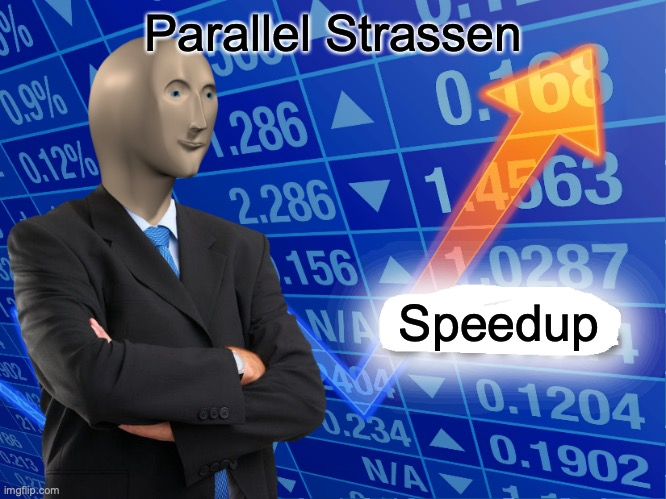
\includegraphics[scale=.5]{58mo62.jpg}}
\caption{Stonks}
\label{fig}
\end{figure}

\section{Introduction}

\section{Algorithms}
In this section all the implemented algorithms are explained in further detail.

\subsection{Matrix Multiplication}

\subsection{Strassen Algorithm}

\subsection{parallel Matrix Multiplication}

\subsection{parallel Strassen Algorithm}

\section{Experiments}

\section{Conclusion}


\if{}

% equation
\begin{align*}
\end{align*}

% vector
\begin{pmatrix}
	x_1 \\
	x_2 \\
	\vdots \\
	x_n
\end{pmatrix}

% matrix
\begin{pmatrix}
			a_{11} & a_{12} & \ldots & a_{1n} \\
			a_{21} & a_{22} & \ldots & a_{2n} \\
			\vdots & \vdots & \vdots & \vdots \\
			a_{m1} & a_{m2} & \ldots & a_{mn}
\end{pmatrix}

%sum
\sum_{i=0}^{n}{}

% list
\begin{itemize}
	\item
	\item
\end{itemize}

\fi{}

\end{document}